\documentclass[12pt, oneside]{book}   	% use "amsart" instead of "article" for AMSLaTeX format
\usepackage{geometry}  
\usepackage{multirow}              		% See geometry.pdf to learn the layout options. There are lots.
\geometry{a4paper}                   		% ... or a4paper or a5paper or ... 
%\geometry{landscape}                		% Activate for rotated page geometry
%\usepackage[parfill]{parskip}    		% Activate to begin paragraphs with an empty line rather than an indent
\usepackage{graphicx}				% Use pdf, png, jpg, or eps§ with pdflatex; use eps in DVI mode
								% TeX will automatically convert eps --> pdf in pdflatex	
\usepackage{amssymb}
\usepackage{fancyhdr}
\usepackage{color}
\usepackage[latin1]{inputenc}
\usepackage{amsmath}
\usepackage[T1]{fontenc}
%SetFonts

%SetFonts
\usepackage{tabularx}

\pagestyle{fancy}
\begin{document}
\thispagestyle{empty}
\hspace{10cm}
Release date 26-02-2016
\\
\\
\begin{center}
{\huge Software Engineering 2:}
{\huge MyTaxiService}
\end{center}
\vspace*{\fill}
\begin{center}
\textbf{\huge Project Plan} 
\\
\large{V2.0}
\end{center}
\vfill
\begin{center}
{\large Dimitar Anastasovski, Marco Colombo}
\end{center}
\clearpage
\tableofcontents
\thispagestyle{empty}
\setcounter{page}{1}
\clearpage
\pagestyle{plain}
\chapter{Introduction}
\section{Purpose}
This project plan documents the project planning process and consists of the following basic tasks:
\begin{itemize}
\item Defining the sequence of tasks to be performed
\item Identifying all deliverables associated with the project
\item Defining the dependency relationship between tasks
\item Estimating the resources required to perform each task
\item Scheduling all tasks to be performed
\item Identifying the known project risks
\item Defining the process ensuring quality of the project product
\item Defining the process specifying and controlling requirements
\end{itemize}
This plan documents and defines the objectives of the project, the approach to be taken, and the commitment being assumed. This document contains the details required to successfully execute the project. Once project execution begins, this plan will be reviewed, baselined, and updated on a regular basis.
\section{Definitions}
\begin{enumerate}
\item \textit{FP:} Function Points
\item \textit{COCOMO:} Constructive Cost Model
\item \textit{ILF:} Internal Logic File
\item \textit{ELF:} External Logic File
\item \textit{EIQ:} External Inquiry
\item \textit{EI:} External Input
\item \textit{EO:} External Output
\item \textit{SLOC:} Source Lines of Code 
\end{enumerate}
\section{Reference documents}
\begin{itemize}
\item Specification Document: myTaxiService Project 
\item Example of usage of FP and COCOMO for Assignment 5
\item Second example of usage of FP and COCOMO for Assignment 5
\end{itemize}
\chapter{Functional Points Approach}
\section{Introduction}
Frequently the term end user or user is used without specifying what is meant. In this case, the user is a sophisticated user. Someone that would understand the system from a functional perspective --- more than likely someone that would provide requirements or does acceptance testing. 

Since Function Points measures systems from a functional perspective they are independent of technology. Regardless of language, development method, or hardware platform used, the number of function points for a system will remain constant. The only variable is the amount of effort needed to deliver a given set of function points; therefore, Function Point Analysis can be used to determine whether a tool, an environment, a language is more productive compared with others within an organization or among organizations. This is a critical point and one of the greatest values of Function Point Analysis.
\begin{figure}[h]
\centering
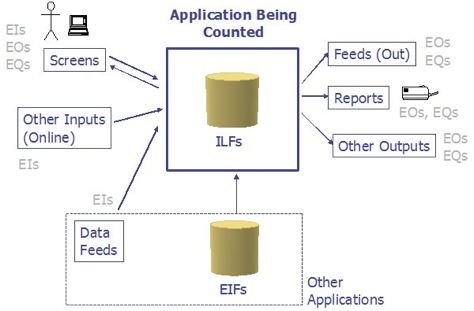
\includegraphics[scale=0.9]{fp.png}
\end{figure}
\\
An ILF is a user-identifiable group of logically related data or control information maintained within the boundary of the application. The primary intent of an ILF is to hold data maintained through one or more elementary processes of the application being counted."
Furthermore, for data or control information to be counted as an ILF, both of the following IFPUG counting rules must also apply:
\begin{enumerate}
\item The group of data or control information is logical and user identifiable.
\item The group of data is maintained through an elementary process within the application boundary being counted.
\end{enumerate}
An external interface file (EIF) is a user identifiable group of logically related data or control information referenced by the application, but maintained within the boundary of another application. The primary intent of an EIF is to hold data referenced through one or more elementary processes within the boundary of the application counted. This means an EIF counted for an application must be in an ILF in another application
\\ \\
An external input (EI) is an elementary process that processes data or control information that comes from outside the application boundary. The primary intent of an EI is to maintain one or more ILFs and/or to alter the behavior of the system.
\begin{figure}[h]
\centering
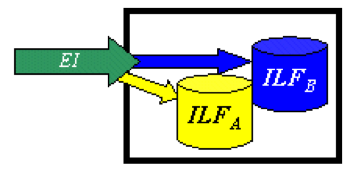
\includegraphics[scale=0.9]{ei.png}
\end{figure}
\\ \\
An external output (EO) is an elementary process that sends data or control information outside the application boundary. The primary intent of an external output is to present information to a user through processing logic other than, or in addition to, the retrieval of data or control information . The processing logic must contain at least one mathematical formula or calculation, create derived data maintain one or more ILFs or alter the behavior of the system. 
\begin{figure}[h]
\centering
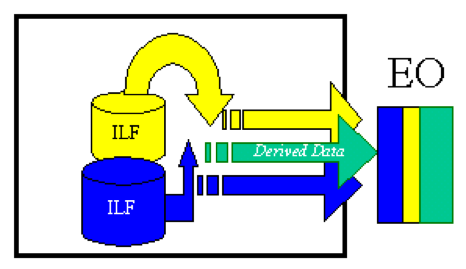
\includegraphics[scale=0.7]{eo.png}
\end{figure}
\\ \\
An external inquiry (EQ) is an elementary process that sends data or control information outside the application boundary. The primary intent of an external inquiry is to present information to a user through the retrieval of data or control information from an ILF of EIF. The processing logic contains no mathematical formulas or calculations, and creates no derived data. No ILF is maintained during the processing, nor is the behavior of the system altered.
\begin{figure}[h]
\centering
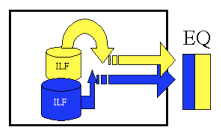
\includegraphics[scale=0.9]{eq.png}
\end{figure}
\section{Function points calculation}
The following table outline the number of Functional Point based on functionality and relative complexity:
\begin{table}[h]
\centering
\begin{tabular}{|c |c |c|c |}
\hline
\multirow{2}{*}{Function Type} & \multicolumn{3}{|c|}{Complexity}\\  \cline{2-4}
&Simple & Medium&Complex\\ 
\hline
\hline
Internal Logic File & 7 & 10 & 15 \\
\hline
External Logic File & 5 & 7 & 10\\
\hline
External Input & 3 & 4 & 6\\
\hline
External Output & 4 & 5 & 7\\
\hline
External Inquiry & 3 & 4 & 6\\
\hline
\end{tabular}
\end{table}
We perform the calculation step by step:
\begin{itemize}
\item \textbf{Internal Logic Files (ILFs):} The application has ILFs, used to store and manage informations about users (Passenger or Taxi Driver), reservation, call and notification.
For notification, call and information about users we can use a simple weight for the not so difficult operation involved. Different case for the reservation that we adopt a complex weight.
\\
So we have: $3 \times 7 +  1 \times 15 = $\textbf{ 36 FPs}
\item \textbf{External Logic Files (ELFs):} The application use two ELFs. One to manage the GPS, using the GoogleMap APIs and the second is the phone company for manage the calls.
These are simple operation so in this case we have: $2 \times 5= $\textbf{ 10 FPs}
\item \textbf{External Input:} The application uses these following inputs:
\begin{itemize}
\item Login/Logout: simple operations so we have $2 \times 3= $\textbf{ 6 FPs}
\item Sign In: This is a simple operation too so $1 \times 3= $\textbf{ 3 FPs}
\item Create a taxi reservation: This is a complex operation because involved more than one entity, so $1 \times 6= $\textbf{ 6 FPs}
\item Change a taxi reservation: This is a complex operation because involved more than one entity, so $1 \times 6= $\textbf{ 6 FPs}
\item Delete a taxi reservation: This is a complex operation because involved more than one entity, so $1 \times 6= $\textbf{ 6 FPs}
\item Call a taxi: This is a simple operation, so $1 \times 3= $\textbf{ 3 FPs}
\item Insert taxi availability: This is a simple operation, so $1 \times 3= $\textbf{ 3 FPs}
\end{itemize}
\item \textbf{External Output:} The application produces the following outputs: 
\begin{itemize}
\item Send a notification to the taxi driver for a desired reservation
\item Send a notification to the passenger to confirm the reservation
\item Call the taxi driver for a ride
\end{itemize}
The first two outputs can considers as medium weight, but the call we can consider is with a simple weight, so we have: $2 \times 5 + 1 \times 4= $\textbf{ 14 FPs}
\item \textbf{External Inquiry:} The application allows user to:
\begin{itemize}
\item View the available taxi for a reservation
\item Change the status of a taxi driver
\end{itemize}
The first can consider as a medium weight, the second as a simple weight.
$1 \times 4 + 1 \times 3= $\textbf{ 7 FPs}
\end{itemize}
In conclusion we have: $36 + 10 + 6 + 3 +6 + 6 + 6 + 3 + 3 +14 + 7 =$\textbf{100 FPs}
\chapter{COCOMO II Approach}
\section{Scale Drivers}
These values are evaluated according to the following table:
\\ \\
\begin{table}[h]
\centering
\begin{tabular}{|p{1.5cm}|p{2cm}|p{2cm}|p{2cm}|p{1.5cm}|p{2cm}|p{2cm}|}
\hline
Scale Factors & \multirow{2}{*}{Very Low} & \multirow{2}{*}{Low} & \multirow{2}{*}{Nominal} & \multirow{2}{*}{High} & \multirow{2}{*}{Very High} & \multirow{2}{*}{Extra High} \\
\hline
PREC \newline \newline SF: & \scriptsize{thorouhly unprecedented} \normalsize{6.20} & \scriptsize{largely unprecedented}  \normalsize{4.96} & \scriptsize{somewhat unprecedented} \normalsize{3.72} & \scriptsize{generally familiar} \normalsize{2.48} & \scriptsize{largely familiar} \newline \newline \normalsize{1.24} & \scriptsize{thoroughly familiar} \newline \normalsize{0.00} \\
\hline
FLEX \newline \newline SF: &  \scriptsize{rigorous}\newline \newline \normalsize{5.07} &  \scriptsize{occasional relaxation} \normalsize{4.05} &  \scriptsize{some relaxation} \normalsize{3.04} &  \scriptsize{general conformity} \normalsize{2.03} &  \scriptsize{some conformity} \newline \normalsize{1.01} &  \scriptsize{general goals} \newline \newline \normalsize{0.00} \\
\hline
RESL \newline \newline SF: &  \scriptsize{little \{20\%\}} \newline \newline \normalsize{7.07} &  \scriptsize{some \{40\%\}} \newline \newline \normalsize{5.65} & \scriptsize{often \{60\%\}} \newline \newline \normalsize{4.24} & \scriptsize{generally \{75\%\}} \normalsize{2.83} & \scriptsize{mostly \{90\%\}} \newline \newline \normalsize{1.41} &  \scriptsize{full \{100\%\}} \newline \newline \normalsize{0.00} \\
\hline
TEAM \newline \newline \newline SF: &  \scriptsize{very difficult interactions} \newline \newline \normalsize{5.46} &  \scriptsize{some difficult interactions} \newline \newline \normalsize{4.38} &  \scriptsize{basically cooperative interactions} \newline \normalsize{3.29} &  \scriptsize{largely cooperative} \newline \newline \normalsize{2.19} &  \scriptsize{highly cooperative} \newline \newline\normalsize{1.10} &  \scriptsize{seamless interactions} \newline \newline \normalsize{0.00} \\
\hline
PMAT \newline \newline SF: &  \scriptsize{SW-CMM Level 1 Lower} \normalsize{7.80} &  \scriptsize{SW-CMM Level 1 Upper} \normalsize{6.24} &  \scriptsize{SW-CMM Level 2} \newline \normalsize{4.68} &  \scriptsize{SW-CMM Level 3} \normalsize{3.12} &  \scriptsize{SW-CMM Level 4} \newline \normalsize{1.56} &  \scriptsize{SW-CMM Level 5} \newline \normalsize{0.00} \\
\hline
\end{tabular}
\end{table}
\begin{itemize}
\item \textbf{Precedentedness:} It reflects the teams previous experience with this kind of projects. Since for this team it was the first experience using this framework and these development methodologies, such as J2EE and Android, this value will be low.
\item \textbf{Development flexibility: }It reflects the degree of flexibility in the development process. The teachers and teaching assistants constructed the assignments giving the general specifications without going too much in details, making this project development very flexible, so, for this reason this value is going to be set to high - general conformity.
\item \textbf{Risk resolution: }Reflects the extent of risk analysis carried out. This value will be high, considering this project.
\item \textbf{Team cohesion: }Reflects how well the development team know each other and work together. Let?s assume that this is team's first project and that they didn't know each other previously. Also, let's assume that there are synchronization problems, such as different academic assignments during project for each of the members. So, this driver will be high - largely cooperative.
\item \textbf{Process maturity: }This was evaluated around the 18 Key Process Area (KPAs) in the SEI Capability Model. 
\newline \newline
There are five levels of process maturity, level 1 (lowest half) to level 5 (highest). The CMM specifies "what" should be in the software process rather than "when" or "for how long".
\newline \newline
The CMM level 1 is for organizations that don't focus on processes or documenting lessons learned. The CMM level 1 is for organizations that have implemented most of the requirements that would satisfy CMM level 2. In CMM's published definition, level 1 (lower half) and (Upper half) are grouped into level 1.
\end{itemize}
\begin{table}[h]
\centering
\begin{tabular}{|c |c |c|}
\hline
Scale Driver & Factor & Value \\
\hline
Precedentedness & Low & 4.96 \\
Development Flexibility & High & 2.03 \\
Risk Resolution & High & 2.83 \\
Team Cohesion & High & 2.19 \\
Process Maturity & High & 3.12\\
\hline
\multicolumn{2}{|c|}{\textbf{Total:}} & 15.13 \\
\hline
\end{tabular}
\end{table}
\section{Cost Drivers}
\begin{itemize}
\item \textbf{Required Software Reliability:} This point is set to Low because in the system occur failures, is possible that some reservation or taxi request are missed.
\begin{figure}[h]
\centering
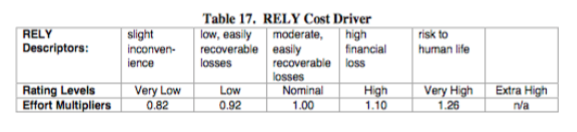
\includegraphics[scale=0.7]{rely.png}
\end{figure}
\item \textbf{DataBase Size:} We can suppose that in our case the rating level could be nominal
\begin{figure}[h]
\centering
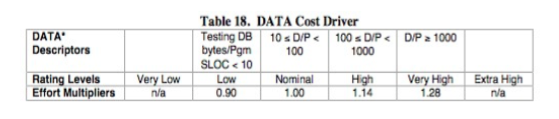
\includegraphics[scale=0.7]{data.png}
\end{figure}
\item \textbf{Product Complexity:} Set to high according to the new COCOMO II CPLEX rating scale
\begin{figure}[h]
\centering
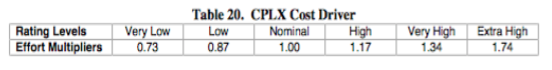
\includegraphics[scale=0.7]{cplex.png}
\end{figure}
\clearpage
\item \textbf{Documentation match to life-cycle need:} is set to nominal because all the aspects are described in the documents.
\begin{figure}[h]
\centering
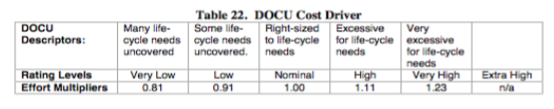
\includegraphics[scale=0.7]{docu.png}
\end{figure} 
\item \textbf{Execution Time Constraint:} In our case is set to very low
\begin{figure}[h]
\centering
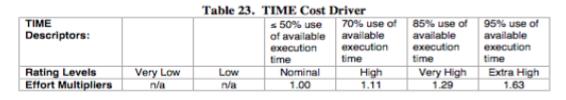
\includegraphics[scale=0.7]{time.png}
\end{figure}
\item \textbf{Main Storage Constraint:} This parameter represents the degree of main storage constraint. In our application this parameter is not relevant so is sets as very low.
\begin{figure}[h]
\centering
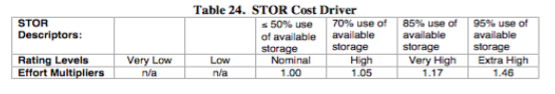
\includegraphics[scale=0.7]{stor.png}
\end{figure}
\clearpage
\item \textbf{Platform Volatility:} We think that this value has to be set to Low
\begin{figure}[h]
\centering
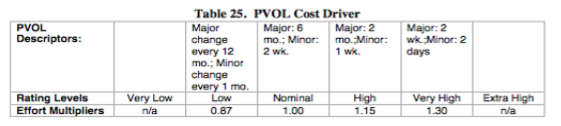
\includegraphics[scale=0.7]{pvol.png}
\end{figure}
\item \textbf{Analyst Capability:} Design and analysis abilities has to be set to High
\begin{figure}[h]
\centering
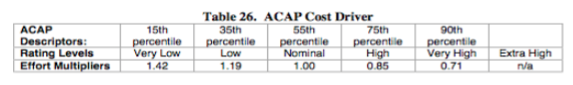
\includegraphics[scale=0.7]{acap.png}
\end{figure}
\item \textbf{Programmer Capability:} This parameter is evaluated according to our degree of cooperation, so it is set to high.
\begin{figure}[h]
\centering
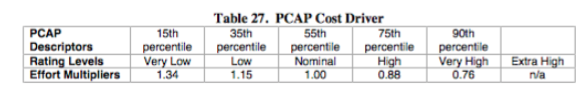
\includegraphics[scale=0.7]{pcap.png}
\end{figure}
\clearpage
\item \textbf{Application Experience:}Since this is our first experience in this typology of project this value is equal to low.
\begin{figure}[h]
\centering
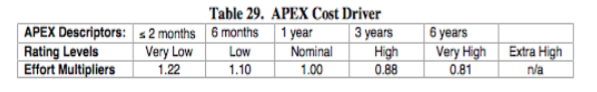
\includegraphics[scale=0.7]{apex.png}
\end{figure}
\item \textbf{Platform Experience:} This parameter is sets as nominal
\begin{figure}[h]
\centering
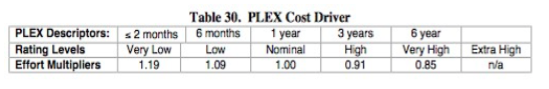
\includegraphics[scale=0.7]{plex.png}
\end{figure}
\item \textbf{Language and Tool Experience:} This parameter is sets as nominal
\begin{figure}[h]
\centering
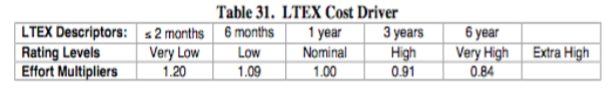
\includegraphics[scale=0.7]{ltex.png}
\end{figure}
\clearpage
\item \textbf{Personnel continuity:} We set this parameter has low 
\begin{figure}[h]
\centering
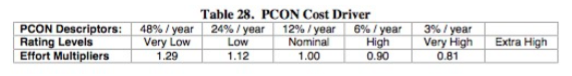
\includegraphics[scale=0.7]{pcon.png}
\end{figure}
\item \textbf{Multisite Development:}This parameter reflects how we handled the distribution of development over distance and multiple platforms. This value is sets to extra high.
\begin{figure}[h]
\centering
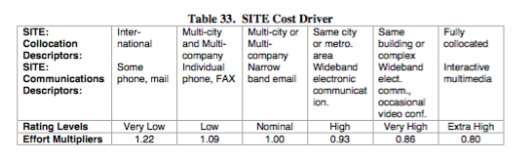
\includegraphics[scale=0.7]{site.png}
\end{figure}
\item \textbf{Required Development Schedule:} We set this parament to high
\begin{figure}[h]
\centering
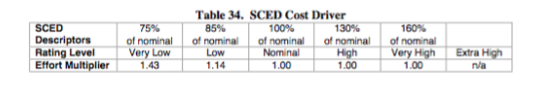
\includegraphics[scale=0.7]{sced.png}
\end{figure}
\end{itemize}
\clearpage
\begin{table}[h]
\centering
\begin{tabular}{|c |c |c|}
\hline
Scale Driver & Factor & Value \\
\hline
RELY & Low & 0.92 \\
DATA & Nominal & 1.00  \\
CPLX & High & 1.17 \\
DOCU & Nominal & 1.00 \\
TIME & Low & n/a \\
STOR & Very Low & n/a \\
PVOL & Low & 0.87 \\
ACAP & High & 0.85 \\
PCAP & High & 0.88 \\
APEX & Low & 1.10 \\
PLEX & Nominal & 1.00 \\
LTEX & Nominal & 1.00 \\
PCON & Low & 1.12 \\
SITE & Extra High & 0.80 \\
SCED & High & 1.00 \\
\hline
\multicolumn{2}{|c|}{\textbf{Total:}} &  0.69\\
\hline
\end{tabular}
\end{table}
\section{COCOMO II calculation}
To pass from FP(Function Points) to SLOC(Source Lines of Code) we use an average conversion factor of 46 lines of code for each function point: \\
$$100 FPs * 46 = 4600 SLOC $$
\\
EAF: Effort Adjustment Factor derived from Cost Drivers. EAF=0.69\\
E:Exponent derived from Scale Drivers. E=0.91 + 0.01*Scale Drivers = 1.0613\\ \\
The formula to calculate the effort is the following:
$$effort = 2.94 * EAF * (KSLOC)^E$$
so we have\\
\centerline{$effort = 2.94 * (0.69) * (4600)^{1.0613} = 10.24$ Person-Months} \mbox{} \\
Now we try to calculate the schedule (duration) of project in month with the following formula\\
\centerline{$Duration = 3.67 * (effort)^{E-0.91}$} \mbox{} \\
we use a new value for E, that is 0.1513. So we have \\ \\
\centerline{$Duration = 3.67 *(10.24)^{0.1513} = 5.21$ Months} \mbox{} \\
\mbox{} \\
Now we can estimate the number of people needed to complete the project with
the following formula: \\ \\
\centerline{$N_{people} = effort / Duration$} \mbox{} \\
\centerline{$N_{people} = 10.24/5.21 = 1.96 \rightarrow 2$ people}
\section{Risk}
A risk is an event or condition that, if it occurs, could have a positive or negative effect on a project's objectives. Risk Management is the process of identifying, assessing, responding to, monitoring and controlling, and reporting risks. This Risk Management Plan defines how risks associated with the MyTaxiService project will be identified, analyzed, and managed. It outlines how risk management activities will be performed, recorded, and monitored throughout the lifecycle of the project and provides templates and practices for recording and prioritizing risks by the Risk Manager and/or Risk Management Team.
\\
\\
\textbf{\large{Risk Assessment}}
\\
\\
Risk assessment is the act of determining the probability that a risk will occur and the impact that event would have, should it occur. This is basically a "cause and effect" analysis. The "cause" is the event that might occur, while the "effect" is the potential impact to a project, should the event occur. Assessment of a risk involves two factors. First is the probability which is the measure of certainty that an event, or risk, will occur. This can be measured in a number of ways, but for the MyTaxiService project will be assigned a probability as defined in the table below.
\\
\begin{table}[h]
\centering
\begin{tabular}{|c|c|c|}
\hline
\multicolumn{3}{|c|}{\textbf{Probability of Occurrences}}\\
\hline
\textbf{Definition} & \textbf{Meaning} & \textbf{Value} \\
\hline
& - Occurs frequently & \\
\textit{Frequent}  &- Will be continuosly experienced unless action & 5 \\
& is taken to change event & \\
\hline
& - Occur less frequently if process is corrected & \\
\multirow{2}{*}{\textit{Likely}} & - Issues identified with minimal audit activity & \multirow{2}{*}{4} \\
& - Process performance failures evident to & \\ 
& trained auditors or regulators & \\
\hline
\multirow{3}{*}{\textit{Occasional}} & - Occurs sporadically & \multirow{3}{*}{3}\\
&-Potential issues discovered during focused & \\
&review&\\
\hline 
\multirow{3}{*}{\textit{Seldom}} & - Unlikely to occur & \multirow{3}{*}{2}\\
& - Minimal issue identification during focused & \\
& review & \\
\hline
\textit{Improbable} & Highly unlikely to occur & 1 \\
\hline
\end{tabular}
\end{table}
\clearpage
\begin{table}[h]
\begin{tabular}{|c|c|c|c|}
\hline
\textbf{Risk} & \textbf{Probability} & \textbf{Effects} & \textbf{Strategy} \\
\hline
\multirow{5}{*}{\textbf{Requirements change}} & \multirow{5}{*}{Moderate} & \multirow{5}{*}{Serious} & Derive traceability \\
& & & information to \\
& & & access requirements to \\
& & & change impact; work on \\
& & & software flexibility\\
\hline
\textbf{Requirements have} & \multirow{8}{*}{Low} & \multirow{8}{*}{Serious} & \multirow{3}{*}{Mention in the beginning} \\
\textbf{compliance  issues} & & &\multirow{3}{*}{what could be legal} \\
 (conflicts) with law & & &\multirow{3}{*}{issues related to requirements} \\
and legal & & & \multirow{3}{*}{and try to reformulate them} \\
regulations - as this  & & &\multirow{3}{*}{in order to avoid conflicts} \\
software deals with  & & & \multirow{3}{*}{with law and legal regulations}\\
personal data which & & & \\
need to be authentic) & & & \\

\hline
\textbf{Requirements fail to}  & \multirow{5}{*}{Moderate} & \multirow{5}{*}{Serious} & \multirow{2}{*}{Involve stakeholders as} \\
 \textbf{align with strategy}  & & & \multirow{2}{*}{much as possible during} \\
 - Requirements conflict & & & \multirow{2}{*}{requirements analysis} \\
with the firm's strategy & & & \multirow{2}{*}{and formulation} \\
(fair taxi managment)  & & & \\
\hline
\multirow{9}{*}{\textbf{Design lacks flexibility}} & \multirow{11}{*}{Moderate} & \multirow{11}{*}{Serious} & Work on training and \\
\multirow{9}{*}{- A poor design makes} & & & improving less  \\
\multirow{9}{*}{change requests difficult} & & & experienced team   \\
\multirow{9}{*}{and costly.} & & &members but,  \\
& &  &in general, let only \\
& & &  the most experienced\\
& & & members do this job,  \\
& & & as design is critical part\\
& & & of the project and is heavily \\
& & & base on experiene with\\
& & & similar projects. \\
\hline
\textbf{Technology components} & \multirow{5}{*}{High} & \multirow{5}{*}{Serious} & Consider different \\
\textbf{aren't scalable} & & & technlogies (as alternatives) \\
- Components that can't & & & and start performance \\
be scaled to meet & & & testing as soon \\
performance demands & & & as possible \\
\hline
\textbf{Technology components} & \multirow{6}{*}{Moderate} & \multirow{6}{*}{Marginal} & \multirow{3}{*}{Use technology that} \\
\textbf{aren't compliant with} & & &\multirow{3}{*}{is already has been} \\
\textbf{standards and best} & & & \multirow{3}{*}{approved as suitable}\\
\textbf{practites} & & & \multirow{3}{*}{for similar systems.} \\
- Non-standard components & & & \\
that violate best practices & & & \\
\hline
\end{tabular}
\end{table}
\clearpage
\begin{table}[h]
\begin{tabular}{|c|c|c|c|}
\hline
\multirow{6}{*}{\textbf{Project team lack}} & \multirow{8}{*}{Low} & \multirow{8}{*}{Catastrophic} & Make clear in the \\
\multirow{6}{*}{\textbf{authority to complete}} & & & beginning what is the \\
& & & authority needed (access \\
& & & to government databases \\
& & & in this case) to complete \\
& & & the project and work on \\
& & & achieving it as early \\
& & & as possible \\
\hline
\multirow{2}{*}{\textbf{Database}} & \multirow{3}{*}{Moderate} & \multirow{3}{*}{Serious} & Consider using\\
\multirow{2}{*}{\textbf{perfomance}} & & & higher perfomance \\
& & & database or cloud \\
\hline
\multirow{7}{*}{\textbf{Junior member not}} & \multirow{8}{*}{Moderate} & \multirow{8}{*}{Catastrophic} & Consider switching other\\
\multirow{7}{*}{\textbf{able to work on mobile app}} & & & team member to this \\
& & & task(either expert or \\
& & & project manager who is not \\
& & & so experienced in mobile \\
& & & apps development but \\
& & & is experienced and educated \\
& & & enough as an engineer to \\
& & & accept such challenge)\\
\hline
\end{tabular}
\end{table}
\clearpage
\section{Task Allocations}
\begin{figure}[h]
\centering
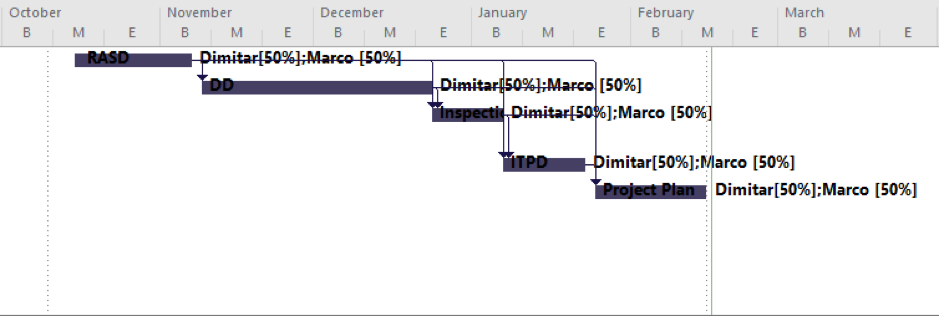
\includegraphics{task.png}
\end{figure}
\vspace{2cm}
\begin{figure}[h]
\centering
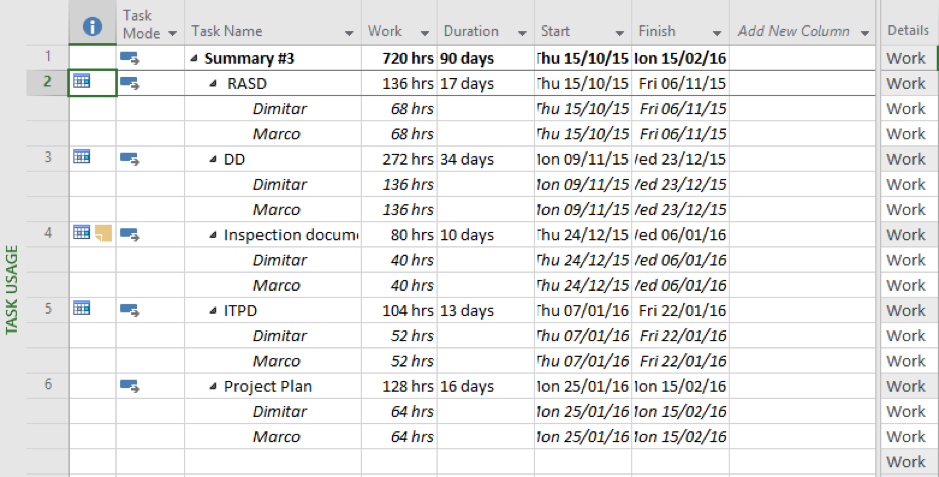
\includegraphics{schedule.png}
\end{figure}
\section{Changelog}
We performed a different calculation for the COCOMO II with the right scale drivers
\end{document}